\begin{problemset}
    \item 直线 $(m-1) x+(m-3) y-2=0$ 与圆 $(x-1)^2+y^2=1$ 的位置关系是 \underline{\qquad}
    \item 图中曲线为圆或半圆，已知点 $P(x, y)$ 是阴影部分（包括边界）的动点，则 $\frac{y}{x-4}$ 的最小值为 \underline{\qquad}
    \begin{figure} [H]
        \centering
        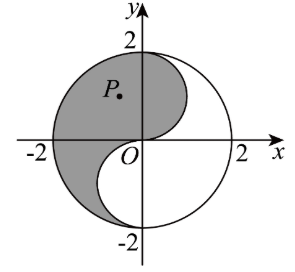
\includegraphics[width=0.2\textwidth]{chapters/直线与圆/images/直线相关的题型/img-20250713004105.png}
    \end{figure}
    \item 已知圆 $C$ 的方程为 $x^2+y^2-2 y-1=0, ~ P(a, b)$ 为圆 $C$ 上任意一点，则 $\frac{2 a+b-5}{a-2}$ 的取值范围为 （\qquad）
    \begin{tasks}(4)
        \task $[-1,2]$
        \task $(-\infty,-1] \cup[2,+\infty)$
                    \task $[1,3]$
                    \task $(-\infty, 1] \cup[3,+\infty)$
    \end{tasks}
    \item 已知点 $P(x, y)$ 是圆 $(x-2)^2+y^2=1$ 上任意一点，则 $\frac{y}{x}$ 的最大值是 （\qquad）
    \begin{tasks}(4)
        \task $\sqrt{3}$
        \task $\frac{\sqrt{3}}{3}$
        \task $\frac{1}{2}$
        \task $\frac{\sqrt{3}}{2}$
    \end{tasks}
    \item 在平面直角坐标系 $x O y$ 中，存在四点 $A(0,1), B(7,0), C(1,0), D(1,3)$ ．
    \begin{enumerate}
        \item 求过三点 $A, B, C$ 的圆 $M$ 的方程，并判断点 $D$ 与圆 $M$ 的位置关系；

        \item 若过点 $D$ 的直线 $l$ 被圆 $M$ 截得的弦长为 8 ，求直线 $l$ 的方程．
    \end{enumerate}
    \item 已知圆 $M$ 过点 $A(1,-3)$、$B(6,2)$ 且圆心在直线 $y=2 x$ 上．
    \begin{enumerate}
        \item 求圆 $M$ 的方程；
        \item 过点 $P(4,-4)$ 的直线 $m$ 被圆 $M$ 截得的弦长为 8 ，求直线 $m$ 的方程．
    \end{enumerate}
    \item 过点 $(-4,3)$ 的圆 $(x+3)^2+(y-1)^2=1$ 的切线方程为 \underline{\qquad}.
    \item 已知圆 $C_1: x^2+y^2+4 x-6 y+4=0$ 与圆 $C_2: 2 x^2+2 y^2=1$ 相交于 $A, B$ 两点，求直线 $A B$ 的方程．
    \item 设 $a$ 为实数，若直线 $2 x+y+a=0$ 与圆 $x^2+y^2-2 x+4 y=0$没有公共点，求 $a$ 的取值范围．
    \item 已知直线 $\sqrt{2} x+y+a=0$ 与 $\odot C: x^2+(y-1)^2=4$ 相交于 $A$、$ B$ 两点，且 $\triangle A B C$ 为等边三角形，则实数 $a=$（\quad）
    \begin{tasks}(4)
        \task -4 或 2
        \task -2 或 4
        \task $-1 \pm \sqrt{3}$
        \task $-1 \pm \sqrt{6}$
    \end{tasks}
\end{problemset}

\subsection{练习答案}
\begin{tips}
    \begin{enumerate}
        \item 直线 $(m-1) x+(m-3) y-2=0$ 与圆 $(x-1)^2+y^2=1$ 的位置关系是 \underline{相交或相切（点在圆上）}
        \item 图中曲线为圆或半圆，已知点 $P(x, y)$ 是阴影部分（包括边界）的动点，则 $\frac{y}{x-4}$ 的最小值为 $-\frac{8}{15}$.
        \item 提示：将 $\frac{2 a+b-5}{a-2}=\frac{2(a-2)+b-1}{a-2}=2+\frac{b-1}{a-2}$
        \item B.
        \item（1）设圆 $M$ 方程为 $x^2+y^2+D x+E y+F=0$
              把 $A, B, C$ 三点坐标代入可得：$\left\{\begin{array}{l}1+E+F=0, \\ 49+7 D+F=0, \\ 1+D+F=0,\end{array}\right.$

              解得 $D=-8, ~ E=-8, ~ F=7$ ，

              所以圆 $M$ 方程是 $x^2+y^2-8 x-8 y+7=0$

              把 $D$ 点坐标代入可得： $1+9-8-24+7<0$ ，故 $D$ 在圆 $M$ 内；

              （2）由（1）可知圆 $M:(x-4)^2+(y-4)^2=25$ ，则圆心 $M(4,4)$ ，半径 $r=5$

              由题意可知圆心到直线 $l$ 的距离是 $\sqrt{5^2-4^2}=3$

              当直线 $l$ 斜率存在时，设直线 $l$ 方程为：$y=k(x-1)+3 \Rightarrow k x-y+3-k=0$

              所以由点到直线的距离公式得 $\frac{|3 k-1|}{\sqrt{1+k^2}}=3$ ，解得 $k=-\frac{4}{3}$ ，故直线 1 的方程为 $4 x+3 y-13=0$ ；

              当直线 $l$ 斜率不存在时，则直线 $l$ 方程为：$x=1$

              此时圆心到直线 $l$ 的距离是 3 ，符合题意．

              综上所述，直线 $l$ 的方程为 $4 x+3 y-13=0$ 或 $x=1$ ．

        \item 圆 $M$ 的方程为 $(x-1)^2+(y-2)^2=25$．

              （2）设圆心 $M$ 到直线 $m$ 的距离为 $d$ ，直线 $m$ 与圆 $M$ 相交于点 $C$、$D$ ，且 $|C D|=8$

              则 $d=\sqrt{r^2-\left(\frac{|C D|}{2}\right)^2}=\sqrt{5^2-4^2}=3^{\prime}$

              又因为直线 $m$ 经过点 $P(4,-4)$

              当直线 $m$ 的斜率不存在时，则直线 $m$ 的方程为 $x=4$

              点 $M(1,2)$ 到 $m$ 的距离为 $|4-1|=3$ ，符合题意；

              当直线 $m$ 的斜率存在时，设直线 $m$ 的方程为 $y+4=k(x-4)$ ，即 $k x-y-4 k-4=0$

              则 $d=\frac{|k-2-4 k-4|}{\sqrt{k^2+1}}=\frac{3|k+2|}{\sqrt{k^2+1}}=3$ ，解得 $k=-\frac{3}{4}$

              此时直线 $m$ 的方程为 $y-2=-\frac{3}{4}(x-1)$ ，即 $3 x+4 y+4=0$.

              所以直线 $m$ 的方程为 $3 x+4 y+4=0$ 或 $x=4$ ．
        \item $x=-4$ 或 $3 x+4 y=0$
        \item $8 x-12 y+9=0$
        \item $(-\infty,-5) \cup(5,+\infty)$（提示：圆心到直线的距离 $d > r$）
        \item A. 提示：圆心到直线的距离为 $d=r \sin 60^{\circ}=\sqrt{3}$.

              即 $d=\frac{|\sqrt{2} \times 0+1+a|}{\sqrt{3}}=\sqrt{3}$ ，整理得 $|1+a|=3$ ，解得 $a=2$ 或 $-4$.
    \end{enumerate}
\end{tips}

\pagebreak
